\documentclass[../main]{subfiles}

\begin{document}

\section{
  Compile time benchmarking: state of the art
}

\cpp \acrfull{tmp} raised interest for allowing computing libraries
to offer great performance with a very high level of abstraction.
Instead of building representations of calculations at runtime for
interpretation, they are built at compile time to be transformed directly into
programs.

As metaprogramming became easier with \cpp11 and \cpp17,
it became more frequent. Consequently developers now have to bear with longer
compilation times, often without being able to explain them.
Therefore being able to measure compilation times becomes increasingly important
and being able to profile and explain them as well.

This need turned into a variety of projects that aim to bring novel techniques
to analyze the compile time performance of \cpp metaprograms and metaprogramming
techiniques beyond black box A/B comparisons.

% \subsection{
%   Build-Bench
% }
%
% Build-Bench\cite{buildbench} measures compiler execution times for basic
% A-B compile time comparisons in a web browser.

\subsection{
  Metabench
}

Metabench\cite{metabench} instantiates variably sized benchmarks using
embedded Ruby (ERB) templating and plots compiler execution time, allowing
scaling analyses of metaprograms. Its output is a series of web-based
interactive graphs.

The ERB templates are used to generate \cpp programs for measuring their
total compilation time. This approach is compiler-agnostic, it allows to compare
not just metaprograms but compilers as well.

However Metabench is currently unmaintained, and its design choices make it
difficult to modify and reuse it for the assessment of metaprogramming
techniques performance in a scientific context:

\begin{itemize}
\item
non-CMake scripts are embedded in CMake strings, making it difficult to modify
and debug them,

\item
benchmarks are not standalone, they are embedded in the Metabench
project itself,

\item
web-based visualizations cannot be embedded in \LaTeX{} documents.
\end{itemize}

\subsection{
  Templight
}

Templight\cite{templight} is the first effort to instrument Clang with a
profiler. It aims to provide tools to measure resource usage (CPU time,
memory usage, and file I/O) of template instantiations.

\subsection{
  Clang's built-in profiler
}

Additionally, Clang has a built-in profiler\cite{time-trace} that provides
in-depth time measurements of various compilation steps, which can be enabled by
passing the \lstinline{-ftime-trace} flag. Its output contains data that can be
directly linked to symbols in the source code, making it easier to study the
impact of specific symbols on various stages of compilation. The output format
is a JSON file meant to be compatible with Chrome's flame graph visualizer, that
contains a series of time events with optional metadata like the mangled \cpp
symbol or the file related to an event. The profiling data can then be
visualized using tools such as Google's Perfetto UI as shown in figure
\ref{fig:perfetto-time-trace-ui}.

\begin{figure}[h]
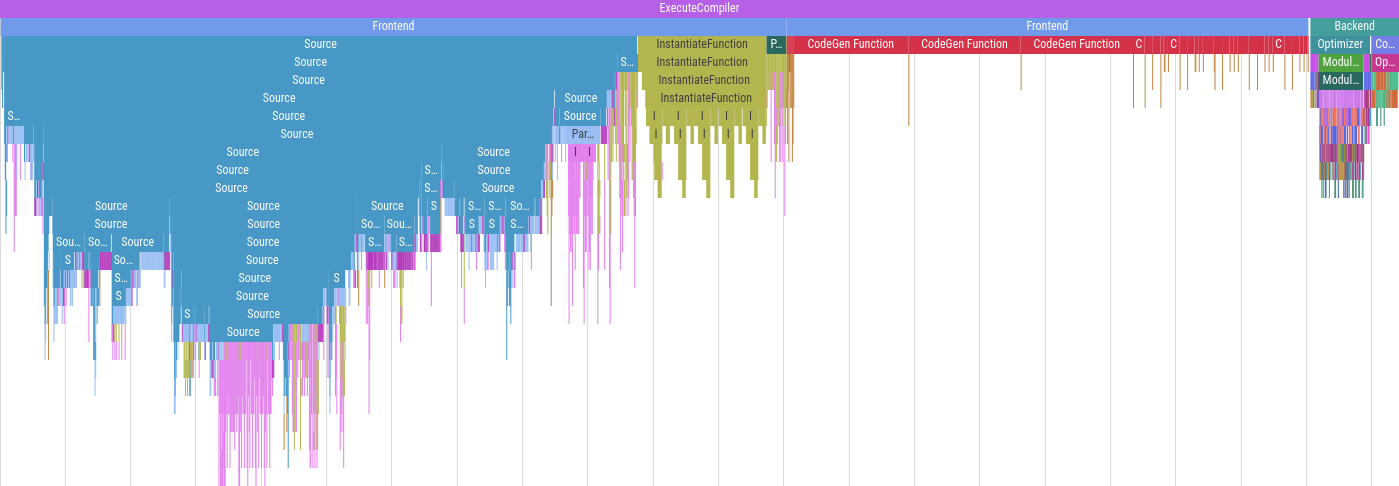
\includegraphics[scale=0.264]{images/perfetto-ui.png}
\caption{Clang time trace file in Perfetto UI}
\label{fig:perfetto-time-trace-ui}
\end{figure}

The JSON files have a rather simple structure. They contain a
\lstinline{traceEvents} field that holds an array of JSON objects, each one of
them containing a \lstinline{name}, a \lstinline{dur} (duration), and
\lstinline{ts} (timestamp) field. It may also contain additional data in the
field located at \lstinline{/args/data}, as seen in listing
\ref{lst:clang-time-trace-event}. Duration and timestamps are expressed in
microseconds.

\begin{lstlisting}[
  language=json,
  caption=Time trace event generated by Clang's internal profiler,
  label=lst:clang-time-trace-event]{}
{
  "pid": 8696,
  "tid": 8696,
  "ph": "X",
  "ts": 3238,
  "dur": 7,
  "name": "Source",
  "args": {
    "detail": "/usr/include/bits/wordsize.h"
  }
}
\end{lstlisting}

In this example the \lstinline{/args/detail} field indicates the file that's
being processed durin this trace event. This field may also contain details
related to symbols being processed for events like
\lstinline{InstantiateFunction}.

Clang's profiler data is very exhaustive and insightful, however there is no
tooling to make sense of it in the context of variable size compile time
benchmarks. \ctbench tries to bridge the gap by providing a tool to analyze
this valuable data. It also improves upon existing tools by providing a solution
that's easy to integrate into existing CMake projects, and generates graphs in
various formats that are trivially embeddable in documents like research papers,
web pages, or documentations. Additionally, relying on persistent configuration,
benchmark declaration and description files provides strong guarantees for
benchmark reproductibility, as opposed to web tools or interactive profilers.

\subsection{
  Conclusion
}

While Metabench could have been a good candidate for assessing the scalability
of metaprogramming techniques, its design choices make it simpler to write a new
tool that better fits the needs of scientific assessment of metaprogramming
techniques.

\ctbench's API and overall concept was largely inspired by this project for its
simplicity and leverages Clang's profiling capabilities that are similar to
those introduced by Templight.

\end{document}
